
\documentclass[a4paper,11pt]{kth-mag}

\usepackage[acronym]{glossaries}
\glsdisablehyper
\usepackage{textcomp}
\usepackage[table]{xcolor}
\usepackage[hidelinks]{hyperref}
\usepackage{todonotes}
\usepackage{lmodern}
\usepackage{amsmath}
\usepackage{amsthm}
\usepackage{url}
\usepackage[swedish,english]{babel}
\usepackage{modifications}
\usepackage{multirow}
\usepackage{textcomp}
\usepackage{listings}
\usepackage{color}
\usepackage{amssymb}
\usepackage{dirtree}
\usepackage{array}
\usepackage{pdfpages}
\usepackage{longtable}
\usepackage[acronym]{glossaries}
\usepackage{graphicx} %To use pictures
\graphicspath{ {images/} }







%\usepackage{comment} % enables the use of multi-line comments (\ifx \fi) 
%\usepackage{fullpage} % changes the margin
%\usepackage[utf8]{inputenc}
%\usepackage[T1]{fontenc}



\makeglossaries
\setlength\parindent{0pt}

\extrafloats{1000}
\bibliographystyle{ieeetran}
\title{Title goes here}
\subtitle{Thesis WIP}
\foreigntitle{Title in Swedish goes here}
\author{Richard Odell}
\date{\today}
\blurb{Master's Thesis at ITM\\Supervisor: Lars Svensson \\ Examiner: Lei Feng}
\trita{TRITA xxx yyyy-nn}


\newacronym{rcv}{RCV}{Research Concept Vehicle}
\newacronym{mpc}{MPC}{Model Predictive Controller}
\newacronym{itrl}{ITRL}{Integrated Transport Research Lab}
\newacronym{pi}{PI}{Proportional-Integral}
\newacronym{abs}{ABS}{Anti-lock Braking System}
\newacronym{dc}{DC}{Direct Current}
\newacronym{pid}{PID}{Proportional-Integral-Derivative}
\newacronym{kth}{KTH}{The Royal Institute of Technology}
\newacronym{mbd}{MBD}{Model-Based Design}





\begin{document}

\frontmatter
\pagestyle{empty}
\removepagenumbers
\maketitle
\selectlanguage{english}


\clearpage
\begin{abstract}

Write the abstract here.

\end{abstract}
\clearpage
\begin{foreignabstract}{swedish}

Abstract in Swedish goes here.

\end{foreignabstract}
\clearpage

\chapter*{Acknowledgements}

I would like to thank...



\glsaddall
\printglossary
\renewcommand{\glsnamefont}[1]{\textbf{#1}}
\printglossary[type=\acronymtype,style=super,nonumberlist,nopostdot,nogroupskip]


\clearpage
\clearpage
\tableofcontents*
\clearpage
\listoffigures*
\clearpage
\listoftables*
\glsaddall



\mainmatter
\pagestyle{newchap}

%%%%%%%%%%%%%%%%  INTRODUCTION   %%%%%%%%%%%%%%%%%%%%%%%

\chapter{Introduction}

This chapter will give an introduction to the thesis. 

\section{Background}

 
The \gls{rcv} at \gls{kth} is a platform for research in vehicle autonomy and vehicle dynamics. For precise autonomous operation, accurate actuation of steering input and wheel torque is critical. The electrical wheel motors of the \gls{rcv} can produce torque for acceleration and braking up to a limit. However, for hard braking maneuvers, regenerative braking is not sufficient and a hydraulic brake system actuated by electric linear actuators is used in addition. In the current configuration, the hydraulic brakes actuate fairly slow (>1s before braking request is met). Thus, a redesign of the control software and the mechanical assembly is needed. The task is challenging due to the non-linear and environment dependent dynamics of the hydraulic system.


\section{Research design/Methodology}
The methodology used for this project will be a case study of how to implement one or more brake controllers, which works best for solving the problem stated together with a comparison of the controllers advantages and disadvantages. The case study will have its focus on qualitative research, as there's extensive work already done within this area. The testing will also have a qualitative orientation in the end to validate the brake model as well as how the controller performs. 

\section{Delimitations}
A lot of aspects affects the behavior of the brakes, and to achieve a properly functioning brake with good reaction time will consume much time. Therefore delimitations must be made in order to make the thesis feasible within the limited time frame. The focus of this thesis will be on making an existing braking system faster in terms of reaction time of reaching the requested braking torque. 

Wheel slip and \gls{abs} are both important factors while designing a modern brake, but this will not be implemented or considered in this thesis due to the fact that there is simply not enough time. Split mu, meaning when there is different friction coefficients acting on the the wheels, for example when one wheel travels over a slip of ice or gravel, will not be considered either. The parts that has been left out will be seen as future work that can be made to further improve the brakes on the vehicle. 
 

\section{Ethics}
Brakes is one of the most vital part to the safety of a vehicle. Although this project handles the brakes while in autonomous drive mode, there will still be one or two people in the car monitoring the autonomous driving, whom might be susceptible to great risks if the brakes do not work. To keep the safety of the vehicle at acceptable levels there is a manual brake pedal that overrides the autonomous drive mode, and brakes the vehicle if necessary. This brake pedal is controlled by the person in the drivers seat, who has experience with the vehicle and is much aware of the risks and behavior of the car. 

The vehicle is not legal to drive in regular traffic, and thus is only driven in big closed off areas, such as a rented runway on Arlanda or in a closed off parking lot, where it is driven at low speeds of up to 45 km/h. The vehicle is also equipped with seat belts dimensioned for racing. 
It is an electric car so the people around wont be exposed to any harmful exhausts. 


\section{Risk assessment}
The risks that is involved with this project include the availability of the \gls{rcv} as well as that ordered hardware gets here on time. Concerning the availability of the \gls{rcv} is mainly concerning test. I do not know how to drive the vehicle or how the whole system works, so I will need help doing the tests. Since the testing phase and later parts of the thesis takes place during summer, I might need to change my plan to match peoples vacation. \newline

Concerning the hardware, the actuators that are mounted on the vehicle is relatively slow, and the system will need to be upgraded to achieve a fast enough response time. The lead times in deliveries must be taken into considerations in the time plan.

\section{Requirements?}

- Speed of the actuators, in ms before request to actual torque meet.

- Should it be optimized for torque meet, or regeneration? that is, should the regenerative me used as torquefill or as main brake? Probably torque fill.

- Maximum negative acceleration/ deceleration.

\section{Outline}
What does the report discuss?
This chapter discusses this, this other chapter discusses that...


%%%%%%%%%%%%%%%%%   BACKGROUND STUDY   %%%%%%%%%%%%%%%%

\chapter{Background study}
This section presents the background study
\section{Frame of reference}
The literature search was done directly in the IEEE Xplore database as well as Google Scholar. The search began with broad definitions as 'braking system autonomous driving' as well as 'braking control methods in autonomous driving', which resulted in a few methods that appeared frequently. These methods where then included in the search, together with searches solely for that method.


\subsection{Hardware setup}
Yu et al. \cite{Yu} discusses differences in a linearly actuated system vs a hydraulic pump system. The linearly actuated system uses a linear actuator that press directly on a hydraulic cylinder, while a hydraulic pump system uses an electric pump to build up pressure and controls the pressure in the system by valves and/or solenoids. The linear actuators are simpler and more fail safe, since it doesn't have as many valves from where there can be a leakage of hydraulic fluid. 


\vspace{5mm}
Line, Manzie and Good \cite{4475522} has constructed a electro-mechanical  brake-by-wire system, which utilizes an electrical motor in the calipers as actuator that controls the pressure between the brake pads and the rotor. There is also a brake pedal that sense the pedal position which in turn sends the brake request to a controller. They compare two different controllers in this paper, a cascaded \gls{pi} controller and a \gls{mpc}. The cascaded \gls{pi} controller has three control loops for force, motor angular velocity and motor current. The \gls{pi} controller works, but due to the systems nonlinearity it is somewhat inconsistent in different situations. The \gls{mpc} performs better in this case, but in order for it to work this efficiently a very good model of the system is needed as ground work, and this might be time consuming. \newline


Xiang et al. \cite{Xiang} writes that a electro-mechanical system is preferable over a electro-hydraulical system, due to the simplicity, the efficiency and stability, the enhanced diagnostic capabilities, cost reduction, space and weight saving as well as the elimination of environmental concerns associated with traditional hydraulic braking systems.\newline

%\vspace{5mm}
Line, Manzie and Good \cite{2004-01-2050} as well as in Ahn et al. \cite{ahn2009analysis} is articles about using a cascaded \gls{pi} controller to control a electro-mechanical brake-by-wire system. Here they present requirements on a electromechanical braking system. They discuss the influence of friction, which makes the system nonlinear. The nonlinearity is discussed in the conclusion, where the nonlinear system is the explanation why the cascaded pi controller does not work as fast in the lower brake pad force spectrum as it does for the higher part of the spectrum. \newline



Frede, Khodabakhshian and Malmquist \cite{Frede460614} has done a state-of-the-art report on by-wire systems, with an extensive part about brake-by-wire. They present an overview of brake blending strategies as well as control strategies to regulate braking torque. Most reports discuss brake blending control, but reports where  brake torque control is achieved by fuzzy logic is presented as well. Isermann \cite{661149} also describes the strengths of a fuzzy logic controller, due to its ability to handle nonlinear systems. \newline

Milan{\'e}s et al. \cite{milanes2010electro} presents in an article how an autonomous braking system is implemented into a ordinary road car. The car is already fitted with a hydraulic braking system with a manually controlled braking pedal, and the autonomous braking system is added on to that, resulting in a electro-hydraulic autonomous braking system similar to that on the \gls{rcv}. 
Although the actuator in this car is a electric pump compared to a linear actuator on the \gls{rcv}, this report shows that a electro-hydraulic system is satisfactory, even though other reports state that electro-mechanical systems are preferable \cite{MechatronicsBook} \cite{Xiang}. \newline

The brake blending will be done by a simple function where the regenerative brakes brakes as much as possible, and when they have reached their maximum braking power, the friction brakes steps in to fill in the missing torque, as described by Troung \cite{truongdevelopment}. \newline


\section{Results/Conclusions from background study}
The results from the literature study is that the two friction brake controllers will consist of a \gls{pid} controller and a fuzzy logic controller. 
The brake blending algorithm will be a simple one where the regenerative brakes brake as much as possible, and the friction brakes fills in the missing torque. 


%%%%%%%%%%%%%%%%%%   IMPLEMENTATION   %%%%%%%%%%%%%%%

\chapter{Implementation}

This chapter could present how the brake is implemented, this in terms of how it is set up in Simulink/Simscape and how the new mounts was made together with why the decision was made to order new ones.

\section{Original setup?}
The friction braking system that is used in the \gls{rcv} in the beginning of this thesis project is a electro hydraulic brake system. The braking system is made up of two linear actuators which are controlled by current from an [escon??] driver, which in turn get its signal from a ---dSpace controller--- (write more about this), which is the main computer in the \gls{rcv}. The linear actuators acts on hydraulic cylinders that transfers the force to the calipers on each wheel, where the force acts on the rotors which brakes the vehicle. The reason there are two linear actuators is due to the fact that there are two completely separated friction braking systems in the vehicle, one system that acts on the two front wheels, and the other that acts on the two rear wheels. This is done to incorporate a higher level of safety, whereas if one of the system breaks down, there will still be braking abilities on two of the four wheels. \newline

There is also a manually operated braking pedal that acts on the hydraulic system, controlling the brakes on all four wheels. This braking pedal which is mechanically connected directly to two hydraulic cylinders is located between the calipers and the hydraulic cylinders connected to the linear actuators. If the manual brake pedal is pressed, the autonomous braking system is mechanically disconnected, and all braking is controlled by the driver. \newline

[Picture of brake system setup]

\section{Brake actuators and other hardware}
At the start of the thesis project the idea was to use the original hardware setup that existed in the \gls{rcv}, but after testing and reading up on the original actuators a decision was made to change to a new set of actuators that are faster and stronger. 

\subsection{Original actuators and lever arm}
The original actuators was of an acme screw type, which involves a lot of friction where up to 80\% of the input power can be dissipated in friction losses [SOURCE]. This means that the motor within the actuator has to work hard to move the rod in each direction. The static friction is also very high, which raises a problem when it come to the control of the actuator. The actuator requires a high current to start moving to overcome the static friction, and when it has overcome that static friction the need of current to keep the motion going is not as high. Thus, the steps in current that is needed to make the actuator move offers a problem in controlling it, since it is hard to control with the step in current that is needed and very small movements in the actuator rod can have large effects to the pressure of the hydraulic system. \\

Although, one feature that could be useful in the acme leadscrew actuators is that the configuration is, within certain forces, self locking. They function in such a way that it moves easily if force is applied from one direction , while if it is applied in the other direction it has to be very high in order for the piston to move. Thus, they can be used as parking brake when the vehicle is turned of, if no other means of parking brake is present. Since the ballscrew actuator has lower internal friction, it cannot be relied upon as parking brake. Though, a parking brake can easily be realized by other means, such as a lever  connected to the manual parking brake etc., and is therefore not included in the scope of this thesis\\

The hardware setup, in terms of mounts and lever arm, that was originally mounted on the \gls{rcv} needed revision as well, especially the lever arms that transferred the force from the actuator to the hydraulic cylinder. As can be seen in picture [SOURCE TO PICTURE], there is a lever arm that transfers the force from actuator to hydraulic cylinder. This arm is over dimensioned, the lever arm is to long. Tests showed that the acme screw actuators reaches their stroke limit when the request for braking torque reaches a certain point, which means that the actuators is able to provide higher force than  originally is possible, hence, the lever arms can be shortened in order to make the system faster while keeping the amount of force that can be delivered. 


\subsection{Mounts for new actuators}

A decision was made to change the original actuators to a pair of new ones. The new actuators are of ball screw type, which incorporate lower friction, both static and dynamic. This will help a lot when constructing the controller for the brakes, since we wont have as high step in the current needed to start moving the actuator rod. \\

New mounts had to be made to fit the new actuators, which are slightly larger than the original lead screw actuators. These mounts where modeled in the 3D CAD program Solid Edge, and can be seen in \ref{fig:CAD_Actuator_mount} [AND MORE]. These parts where then manufactured by water jet cutting by the machine department at \gls{kth}. The parts that where constructed where new mounts to the actuators, mounts to the hydraulic cylinders as well as a new connection between the actuator and lever arm. The hydraulic cylinders has not been changed during the thesis project, but since the actuator mounts has been made wider as the actuators are wider, the cylinders had to be wider apart as well to get everything to line up properly. \\

The connection between the actuator and lever arm was made with regards to the possibility to change the position of the connection on the lever arm, to be able to change the leverage. The connection consists of a T-shaped part that is mounted on the actuator while also clamping on to the lever arm with the help of another piece of metal with holes drilled, two screws and bolts. \\

\begin{figure}[h]
\centering
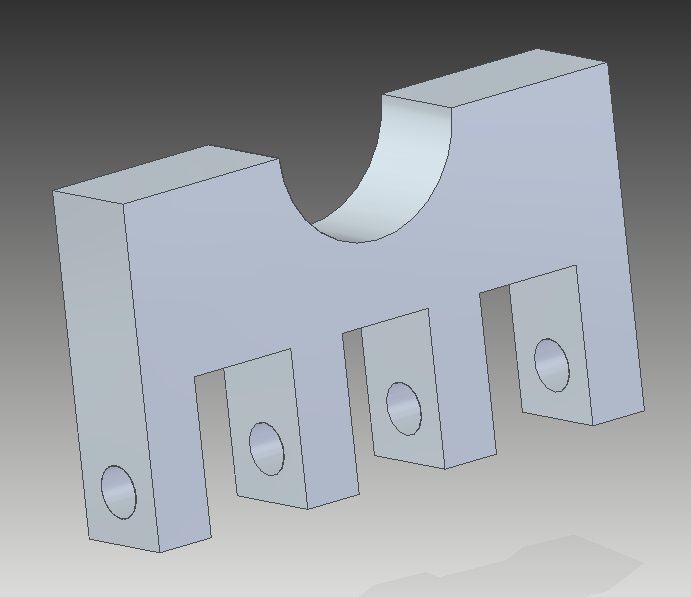
\includegraphics[width=0.5\textwidth]{Actuator_mount}
\caption{CAD picture of mount}
\label{fig:CAD_Actuator_mount}
\end{figure}

\begin{figure}[h]
\centering
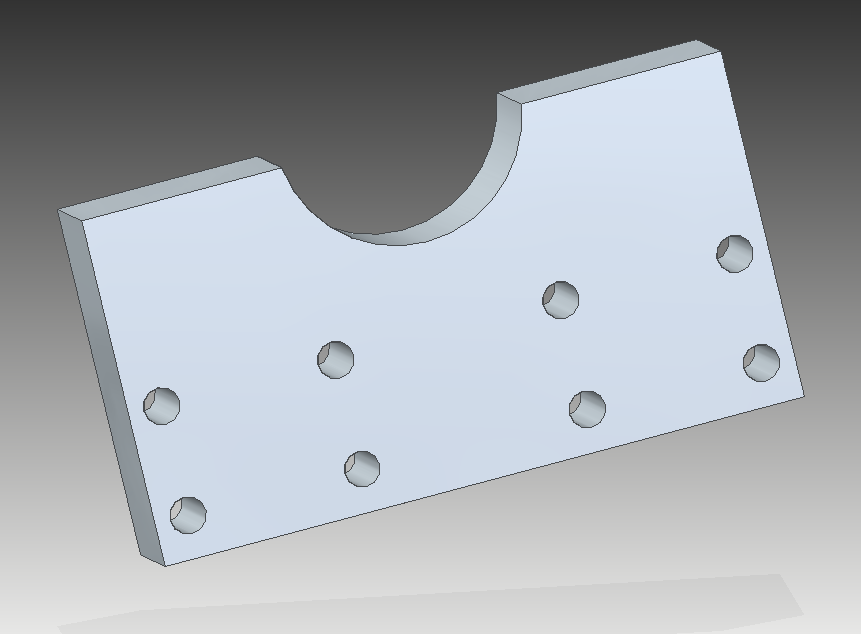
\includegraphics[width=0.5\textwidth]{Hydraulic_cylinder_mount}
\caption{CAD picture of the hydraulic cylinder mount}
\label{fig:CAD_Hydraulic_cylinder_mount}
\end{figure}



\section{Implementation and tuning in simulink/simscape}

The development of the controller was made using \gls{mbd}, where the model was made using the graphical programming environment Simulink. Primarily the tool box Simscape was used, which is a tool box useful while designing physical systems. The model was then VERIFIED, and used while tuning the brake controller. 

\subsection{Simscape model (and MBD?)}
The plant model was constructed in Simulink, mostly using the Simscape toolbox. The plant is made up of a few different parts which are the hydraulic system, the brake calipers, electric actuators and mechanical force translation such as lever arm. All of these parts are made up of Simscape blocks that are tuned by measured or calculated values  as well as values derived from data sheets. The choice of using \gls{mbd} was due to the fact that it is an easy and fast. 

This way of solving a problem by making a software plant model and designing the controller from there is called \gls{mbd}, which has become a very popular method of solving engineering problems, since when a plant model has been made it is easy, fast and cheap to develop and improve the controls\cite{2010-01-1999}. 

\subsection{Verification of simscape model}
When the simscape model was done the plant need to be verified before the of the controlled is done. The verification was made by running the physical system with the new actuators and all necessary hard ware mounted at certain current requests and the compare the results with from the same cases of current request on the plant model. The results can be seen in [FIGURE]. 

\subsection{Tuning controller}
The \gls{pid} controlled was tuned using pole placement design. \\

A feed forward was also incorporated\\

Something about anti windup\\

%%%%%%%%%%%%%   RESULTS   %%%%%%%%%%%%%%%%%%%%


\chapter{Results}
This chapter presents the results of the thesis.
\section{Hardware}
The highest needed braking torque on each wheel was calculated with respect to the maximum negative acceleration that is stated in the requirements. If the acceleration is known, as well as the mass of the vehicle the total force that needs to act on the vehicle can be calculated with Newtons second law, 
\begin{equation}
F_{tot}=m\cdot a,
\end{equation}
where $F_{tot}$ is the total force needed to achieve acceptable deceleration, $m$ is the mass of the vehicle and $a$ is the acceleration. The vehicle has four wheels and the force is considered to be divided evenly distributed on each wheel. Hence, this gives us 
\begin{equation}
F_{wheel}=\frac{F_{tot}}{4},
\end{equation}
where $F_{wheel}$ is the force needed on each wheel. The torque needed on that wheel can then be calculated by 
\begin{equation}
M=F_{wheel}\cdot r,
\end{equation}
where $M$ is the torque and $r$ is the radius of the wheel. The required torque on each wheel was calculated to 350 Nm.



%%%%%%%%%%%%%%%   CONCLUSION   %%%%%%%%%%%%%%%%%%

\chapter{Conclusion}
This is what a chapter looks like.
%%%%%%%%%%%%%%%   DISCUSSION   %%%%%%%%%%%%%%%%%%

\chapter{Discussion}
This is what a chapter looks like.
%%%%%%%%%%%%%%%   FUTURE WORK   %%%%%%%%%%%%%%%%%%

\chapter{Future work}
This is what a chapter looks like.


%%%%%%%%%%%%%%%   REFERENCES   %%%%%%%%%%%%%%%%%%


\bibliography{mybib}
\appendix
\addappheadtotoc
\chapter{First Appendix}

Appendix text goes here.
\glsaddall
\end{document}
